\chapter{Spleckle y procesamiento}

Esta clase tiene como objetivo comprender los pasos básicos de preprocesamiento de imágenes SAR. Para ello se descargarán imágenes de la web y se procesarán a distintos niveles de corrección geométrica y radiométrica.

\section{Descarga de imágenes}

Para descargar imágenes SAR utilizaremos el catálogo del \href{https://vertex.daac.asf.alaska.edu/}{Alaska Satellite Facility}\footnote{\href{https://vertex.daac.asf.alaska.edu/}{https://vertex.daac.asf.alaska.edu/}}. Diríjase a la página y en la sección de \emph{Geographic Region} seleccione un área que incluya a la ciudad de Ushuaia (Figura \ref{fig:region}).

\begin{figure}[h!]
    \centering
    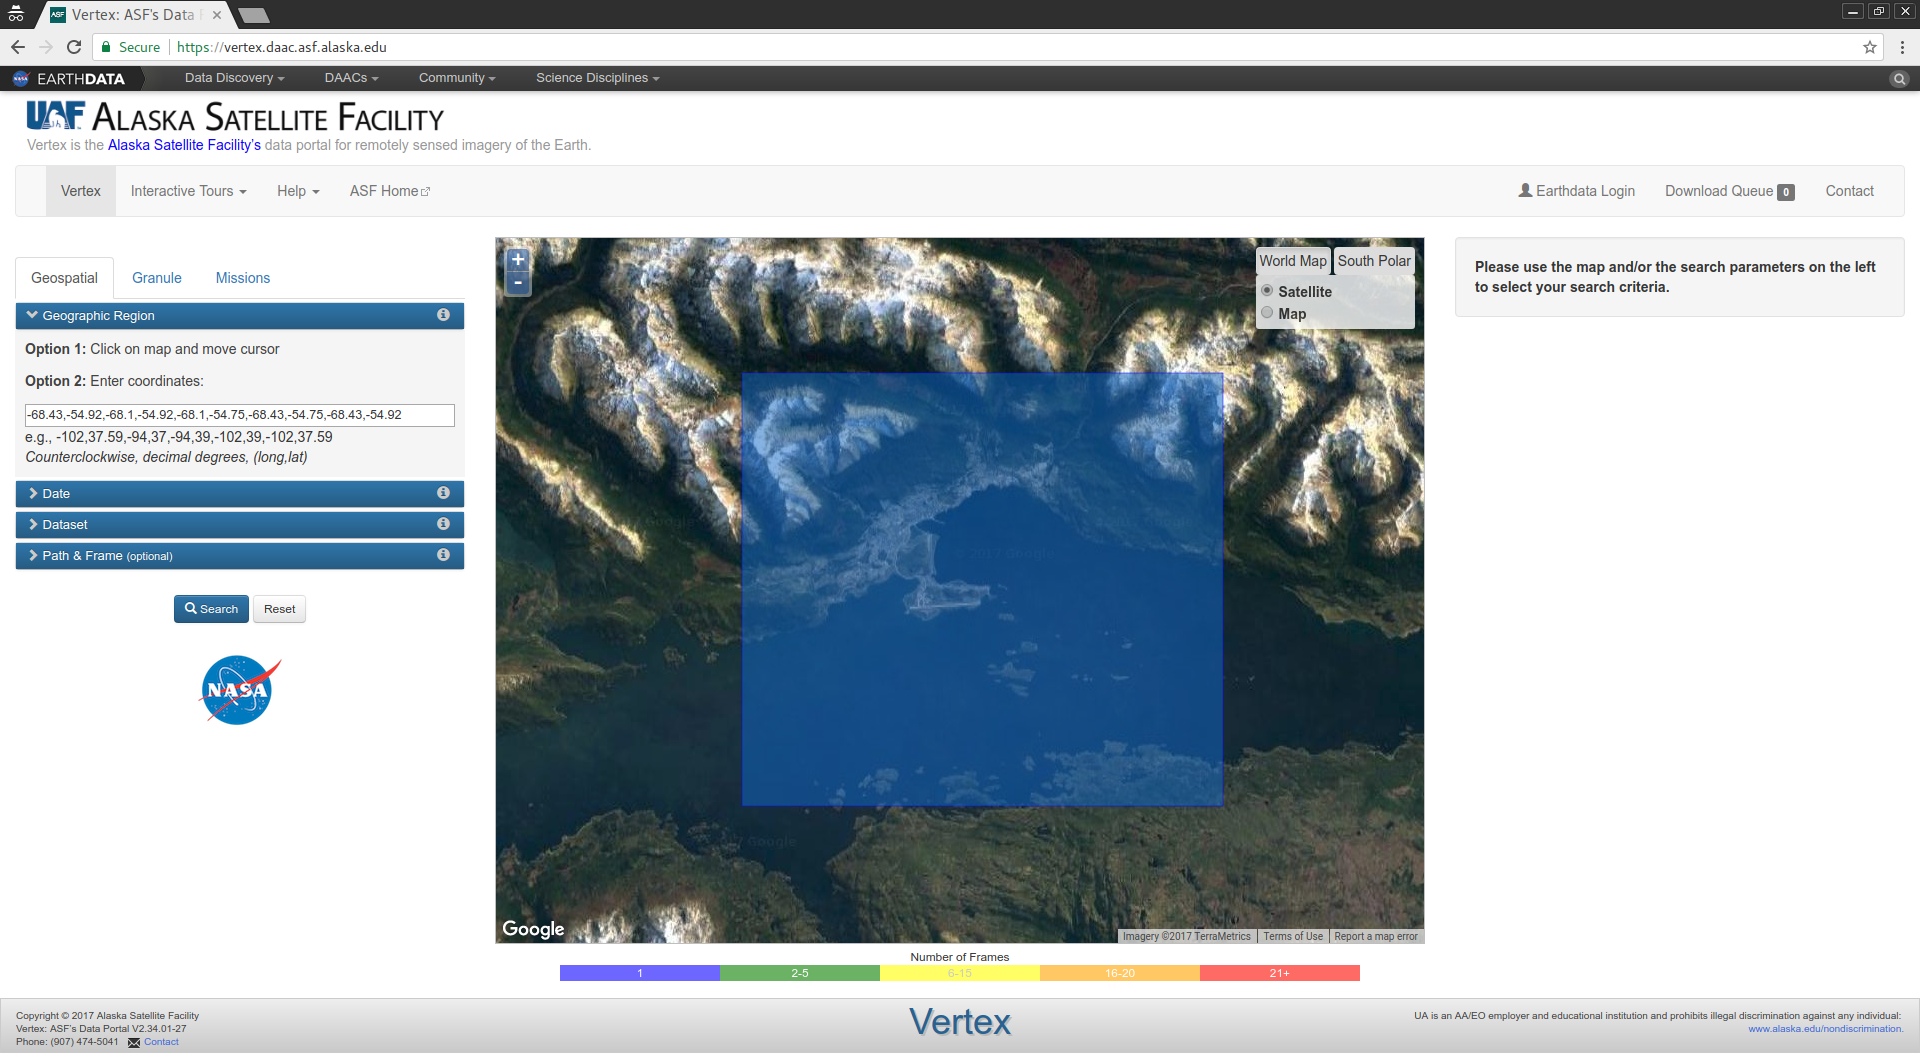
\includegraphics[width=0.8\textwidth]{fig:region.png}
    \caption{Selección de un área de interés en el catálogo \emph{Vertex} del \emph{Alaska Satellite Facility}}
    \label{fig:region}
\end{figure}

Seleccione en \emph{Dataset} el set de datos de \emph{ALOS PALSAR} (Figura \ref{fig:dataset}) y presione search.

\begin{figure}[h!]
    \centering
    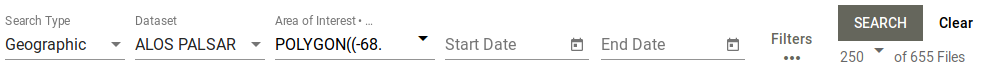
\includegraphics[width=0.8\textwidth]{fig:dataset.png}
    \caption{Selección de \emph{Dataset} en el catálogo \emph{Vertex} del \emph{Alaska Satellite Facility}}
    \label{fig:dataset}
\end{figure}

A la derecha de la pantalla aparecerá una lista de productos. Seleccione de ellos el de nombre \emph{ALOS PALSAR PLR} del 20 de abril del 2011, pertenenciente al frame 6070 y el path 119 (Figura \ref{fig:descarga}).

Descarge el producto \emph{Level 1.1 Complex (661.42 MB)} (Figura \ref{fig:descarga}). En caso de que el sistema así se lo pida, regístrese.

\begin{figure}[h!]
    \centering
    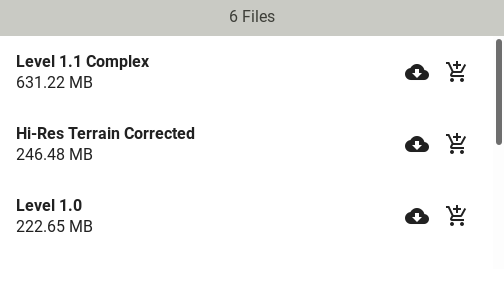
\includegraphics[width=0.8\textwidth]{fig:descarga.png}
    \caption{Slección de producto para la descarga en el catálogo \emph{Vertex} del \emph{Alaska Satellite Facility}}
    \label{fig:descarga}
\end{figure}

El producto descargado corresponde a una imagen \emph{Single look complex} en \emph{slant range}.

\section{Calibración}

Abra la imagen \directory{ALPSRP278916070-L1.1.zip} en SNAP. Despliegue la banda \path{intensity_HH} y observe que se encuentra comprimida horizontalmente.

Para calibrar la imagen, dirijase al menu \menu{Radar>Radiometric>Calibrate} (Figura \ref{fig:calibrar}) y asigne una ruta de guardado.

 \begin{figure}[h!]
     \centering
     \subfloat[I/O Parameters]{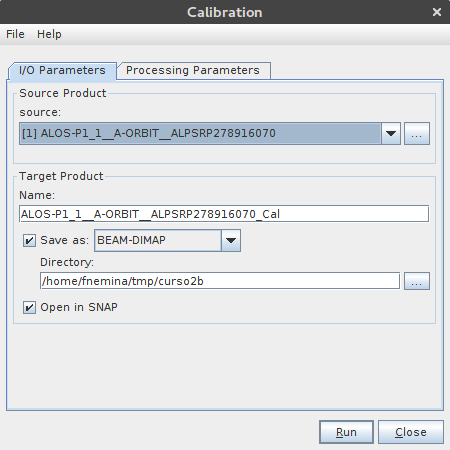
\includegraphics[width=0.35\textwidth]{fig:calibrar1.png}}
     \hfill
     \subfloat[Processing parameters]{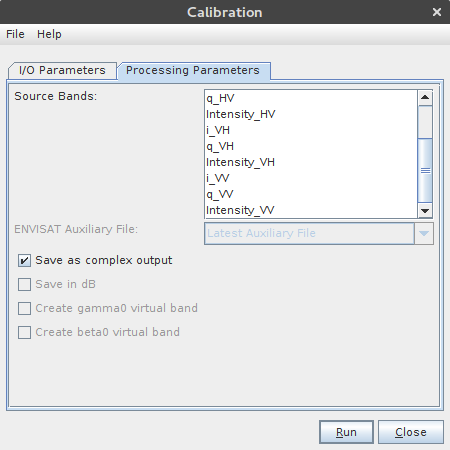
\includegraphics[width=0.35\textwidth]{fig:calibrar2.png}}
     \caption{Calibración de productos SAR utilizando el SNAP. Recuerde seleccionar el directorio de salida en \emph{Directory}.} % arreglar figura
     \label{fig:calibrar}
 \end{figure}

 Obtendrá una imagen con los coeficientes de backscatter \path{sigma_0}. En este caso tendrá las bandas correspondientes a las 4 formas de interacción entre el blanco y la radiación (HH, HV, VH y VV). Este tema será desarrollado en la próxima clase.

 \section{Filtrado}

 Para disminuir el ruido speckle en la imagen se pueden realizar dos procesos distintos.

 \subsection{Multilooking}

 El multilooking genera una nueva imagen a partir de los píxeles en una ventana. Para realizarlo utilice la herramienta \menu{Radar>Multilooking}.

 En source seleccione la imagen \directory{ALOS-P1\_1\_\_A-ORBIT\_\_ALPSRP278916070\_Cal} que generó en el paso anterior. La solapa Processing Parameters permite indicar el numero de looks y sobre que bandas se ejecutará; de no seleccionar ninguna, el proceso se realizará sobre todas las bandas. En éste caso utilice 1 look y la totalidad de las bandas de la imagen (Figura \ref{fig:multilook}).

\begin{figure}[h!]
    \centering
    \subfloat[I/O Parameters]{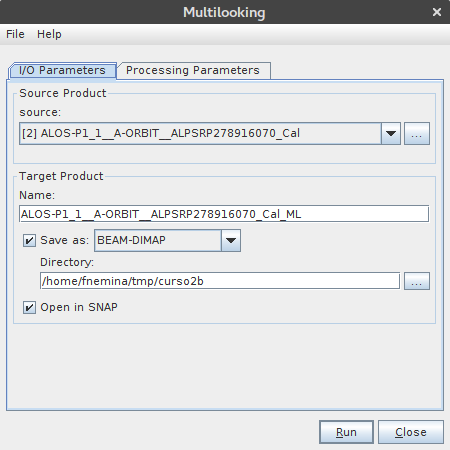
\includegraphics[width=0.35\textwidth]{fig:multilook1.png}}
    \hfill
    \subfloat[Processing parameters]{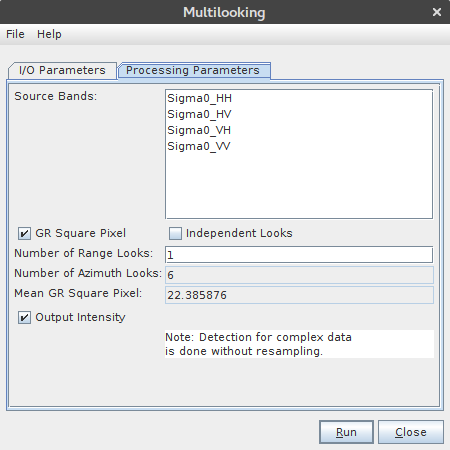
\includegraphics[width=0.35\textwidth]{fig:multilook2.png}}
    \caption{Multilook de una imagen SAR utilizando el SNAP.}
    \label{fig:multilook}
\end{figure}

\begin{que}
Observe la banda \path{sigma_0_HH} de la imagen obtenida.
\end{que}


\subsection{Speckle filter}

Existen otros filtros que ayudan a disminuir el ruido de la imagen. Uno de los más comunes es  \menu{Lee Sigma}, que se encuentra en el menú \menu{Radar>Speckle Filter>Single Product Speckle Filter}.

\begin{figure}[h!]
    \centering
    \subfloat[I/O Parameters]{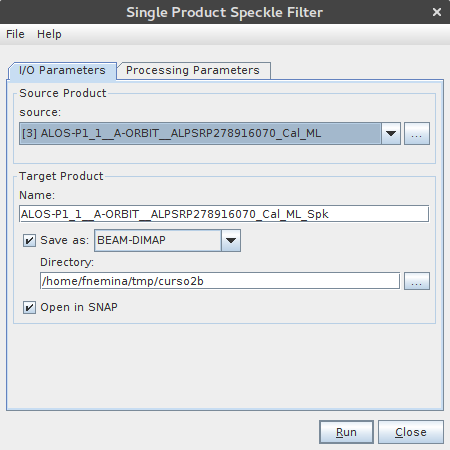
\includegraphics[width=0.35\textwidth]{fig:lee1.png}}
    \hfill
    \subfloat[Processing parameters]{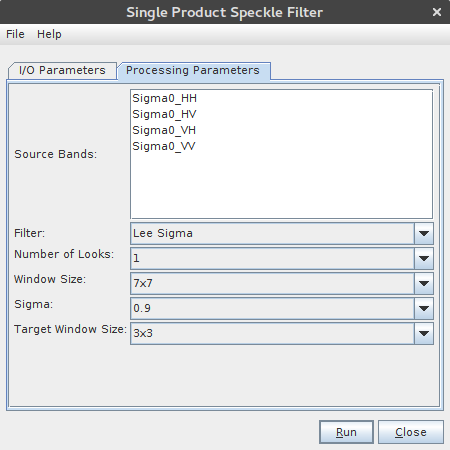
\includegraphics[width=0.35\textwidth]{fig:lee2.png}}
    \caption{Filtrado para reducir el ruido Speckle utilizando el filtro \emph{Lee Sigma}.}
    \label{fig:lee}
\end{figure}

SEn I/O Parameters, source seleccione la imagen \directory{ALOS-P1\_1\_\_A-ORBIT\_\_ALPSRP278916070\_Cal\_ML} que generó al aplicar el multilook. En processing parameter, elija el filtro de \menu{Lee Sigma} con un número de looks igual a 1 y una ventana de 7x7 (Figura \ref{fig:lee})



\begin{que}
    Observe y compare la banda \path{sigma_0_HH} de la imagen con y sin filtro.
\end{que}

\section{Proyección}

Finalmente, es común proyectar la imagen del \emph{slant range} al \emph{ground range}, para que luego se pueda abrir en cualquier softwarae de GIS sin problemas. Existen dos opciones: proyectar la imagen sobre el elipsoide o sobre un modelo de elevación digital.

Para las imágenes ALOS PALSAR 1, es necesario aplicar un proceso antes de proyectarla en el terreno, denominado \emph{deskewing}. En el menú \menu{Radar>Geometric>ALOS deskewing} ejecute el proceso sobre la imagen \directory{ALOS-P1\_1\_\_A-ORBIT\_\_ALPSRP278916070\_Cal\_ML\_Spk}, sin modificar los parámetros por defecto.

\subsection{Elipsoide - GEC}

Al proyectar la imagen sobre el elipsoide podrá hacerlo sobre cualquier lugar del planeta pero, en este caso, no estará utilizando la información del relieve. % ver si se entiende

Para hacerlo, vaya al menú \menu{Radar>Geometric>Ellipsoid Correction>Average Height Range Doppler}. Seleccione la imagen \directory{ALOS-P1\_1\_\_A-ORBIT\_\_ALPSRP278916070\_Cal\_ML\_Spk\_DSk} y deje los parametros por defecto (Figura \ref{fig:elipsoide}).

\begin{figure}[h!]
    \centering
    \subfloat[I/O Parameters]{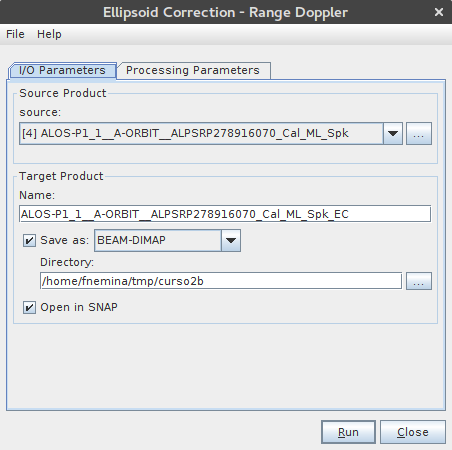
\includegraphics[width=0.35\textwidth]{fig:elipsoide1.png}}
    \hfill
    \subfloat[Processing parameters]{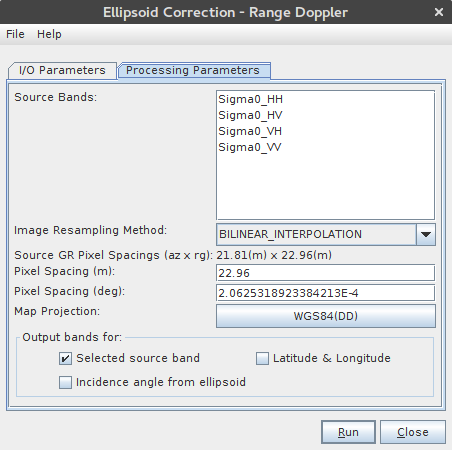
\includegraphics[width=0.35\textwidth]{fig:elipsoide2.png}}
    \caption{Proyección de un producto SAR sobre el elipsoide.}
    \label{fig:elipsoide}
\end{figure}

\begin{que}
    ¿Qué sucede con la imagen luego de la proyección?
\end{que}

\subsection{Elipsoide - GTC}

Al proyectar la imagen sobre un modelo de elevación digital está teniendo en cuenta el relieve del lugar, mejorando algunos aspectos de la imagen como el forshortening y el foreshadowing.

Para hacerlo, vaya al menú \menu{Radar>Geometric>Terrain Correction>Range Doppler Terrain Correction}. Seleccione la imagen \directory{ALOS-P1\_1\_\_A-ORBIT\_\_ALPSRP278916070\_Cal\_ML\_Spk\_DSk} y en \menu{processing parameters} destilde la opción \emph{Mask out areas without elevation} (Figura \ref{fig:gtc}).

{\bf Importante:} Al realizar la proyección sobre un DEM el SNAP lo descarga automaticamente. Esto puede tomar varios minutos dependiendo de su conexión.

\begin{figure}[h!]
    \centering
    \subfloat[I/O Parameters]{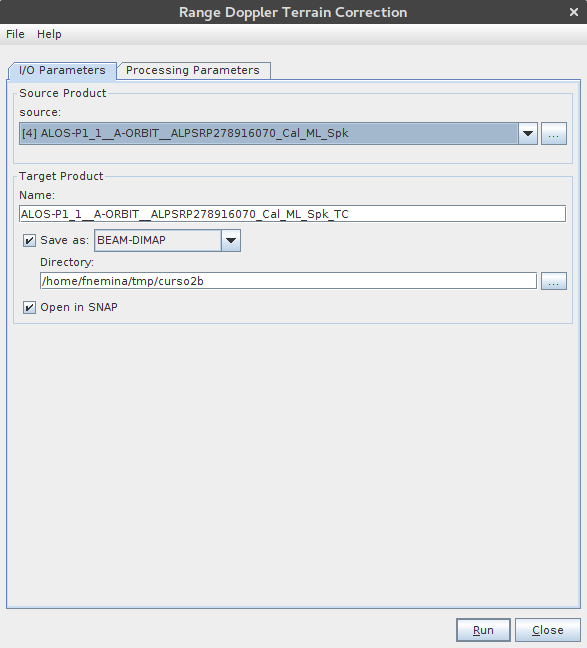
\includegraphics[width=0.35\textwidth]{fig:gtc1.png}}
    \hfill
    \subfloat[Processing parameters]{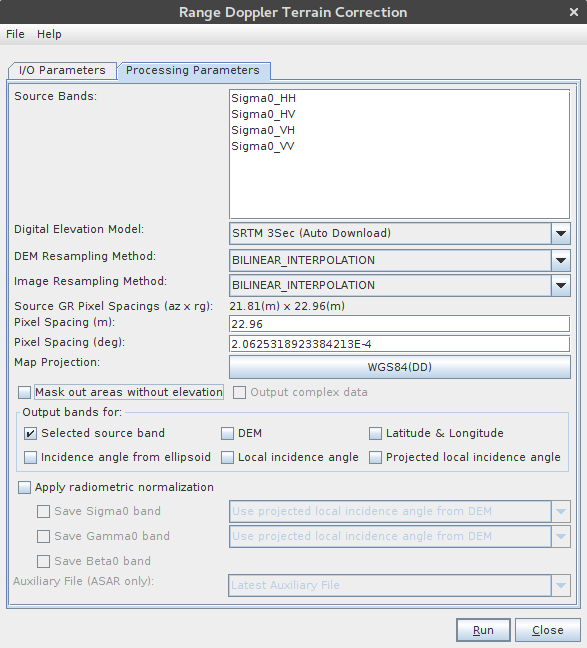
\includegraphics[width=0.35\textwidth]{fig:gtc2.png}}
    \caption{Proyección de un producto SAR sobre un DEM.}
    \label{fig:gtc}
\end{figure}

\begin{que}
    ¿Qué sucede con la imagen luego de la proyección?
\end{que}

\section{dB}

Puede convertir la imagen a dB haciendo click derecho sobre la banda y seleccionando la opción \menu{Linear to/from dB}.

Convierta a dB la banda \path{sigma_0_HH} y explore visualmente el resultado. Conviene siempre explorar las imagenes en dB pues es una medida más natural para nuestro ojo. Sin embargo, al momento de realizar procesamiento, conviene utilizar la imagen sin hacerlo. % yo no pondria ese parrafo y agrgaria una pregunta: cómo observa la imagen, que diferencias encuentra?

\section{Actividades}

\begin{que}
    Compare visualmente las imágenes TC y EC obtenidas por los métodos anteriores. ¿Qué sucede con las montañas? ¿Hacia donde parecen estar inclinadas?
\end{que}

\begin{que}
    ¿Por qué las montañas parecen mas brillantes de un lado que del otro?
\end{que}

\begin{que}
    Obtenga los valores de dB para las coberturas de agua, urbano y bosque.
\end{que}

\begin{que}
    Dentro del agua encontrará un punto muy brillante cerca de la ciudad de Ushuahia. ¿A qué se debe este punto? ¿Qué aplicación le encuentra a las imágenes SAR para detectar objetos sobre el agua?
\end{que}
